\section{Measurement Results and Evaluation}

\subsection{Calibration of the setup with spectra of sodium and mercury}


The calibration of the setup has been carried out measuring the positions of known lines of Sodium and Mercury
(\autoref{img:na:spectrum} and \autoref{img:hg:spectrum}).
The measured data matches the literature values already well.
However, as a small offset is visible over the measured range, a linear fit has been done
to correct the data of the iodine absorption.
The fit and the fitting parameters are shown on \autoref{img:calibrationsystem}.

Furthermore the shortening of the measured wavelengths, which is caused by air, needs to be considered.
Hence a linear fit on the literature values of the refractive index of air has been done and provides another
correcting function which is applied on the measured data for iodine.

\begin{figure}[H]
\begin{center}
  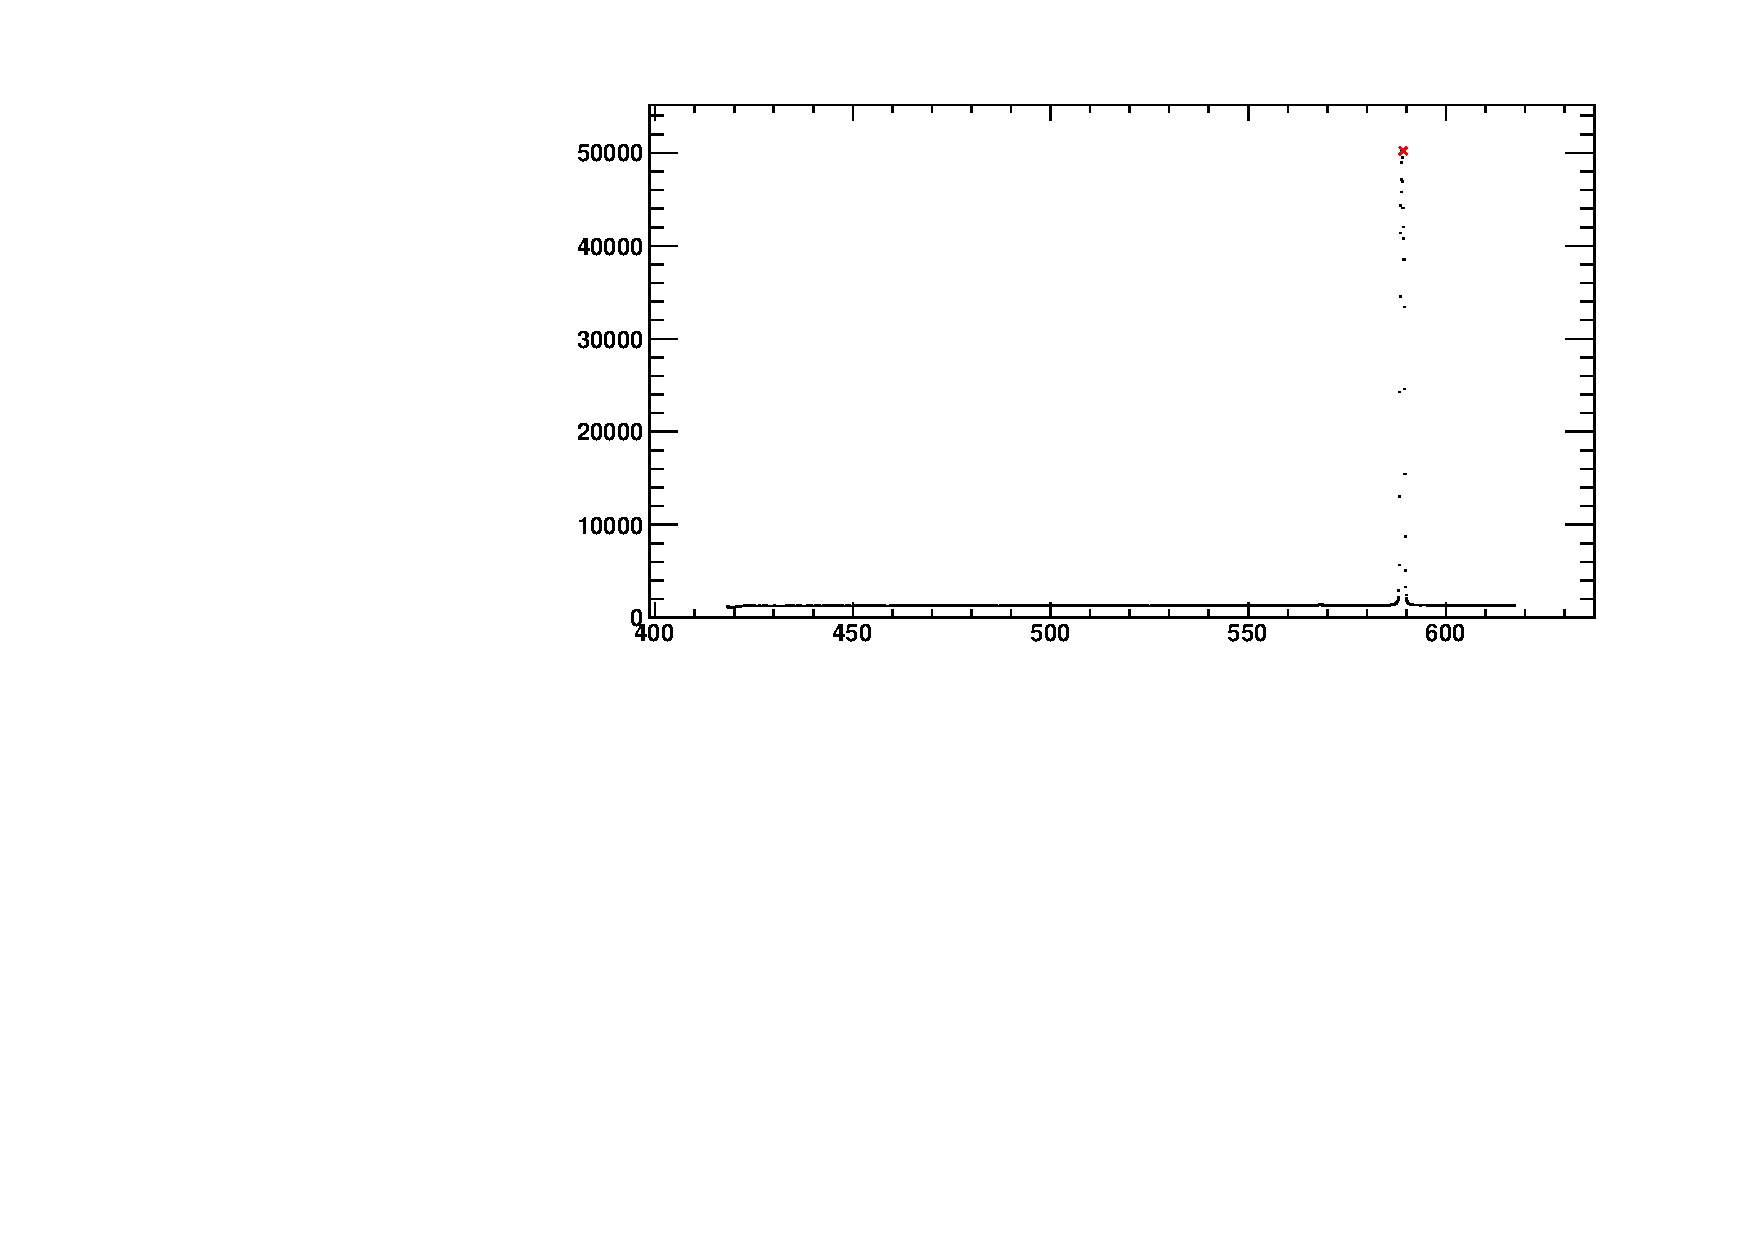
\includegraphics[width=\textwidth]{../img/NaPeaks.pdf}
  \caption[---]{Emission spectrum of Sodium with D-line at 589.20\,nm.}
  \label{img:na:spectrum}
\end{center}
\end{figure}

\begin{figure}[H]
\begin{center}
  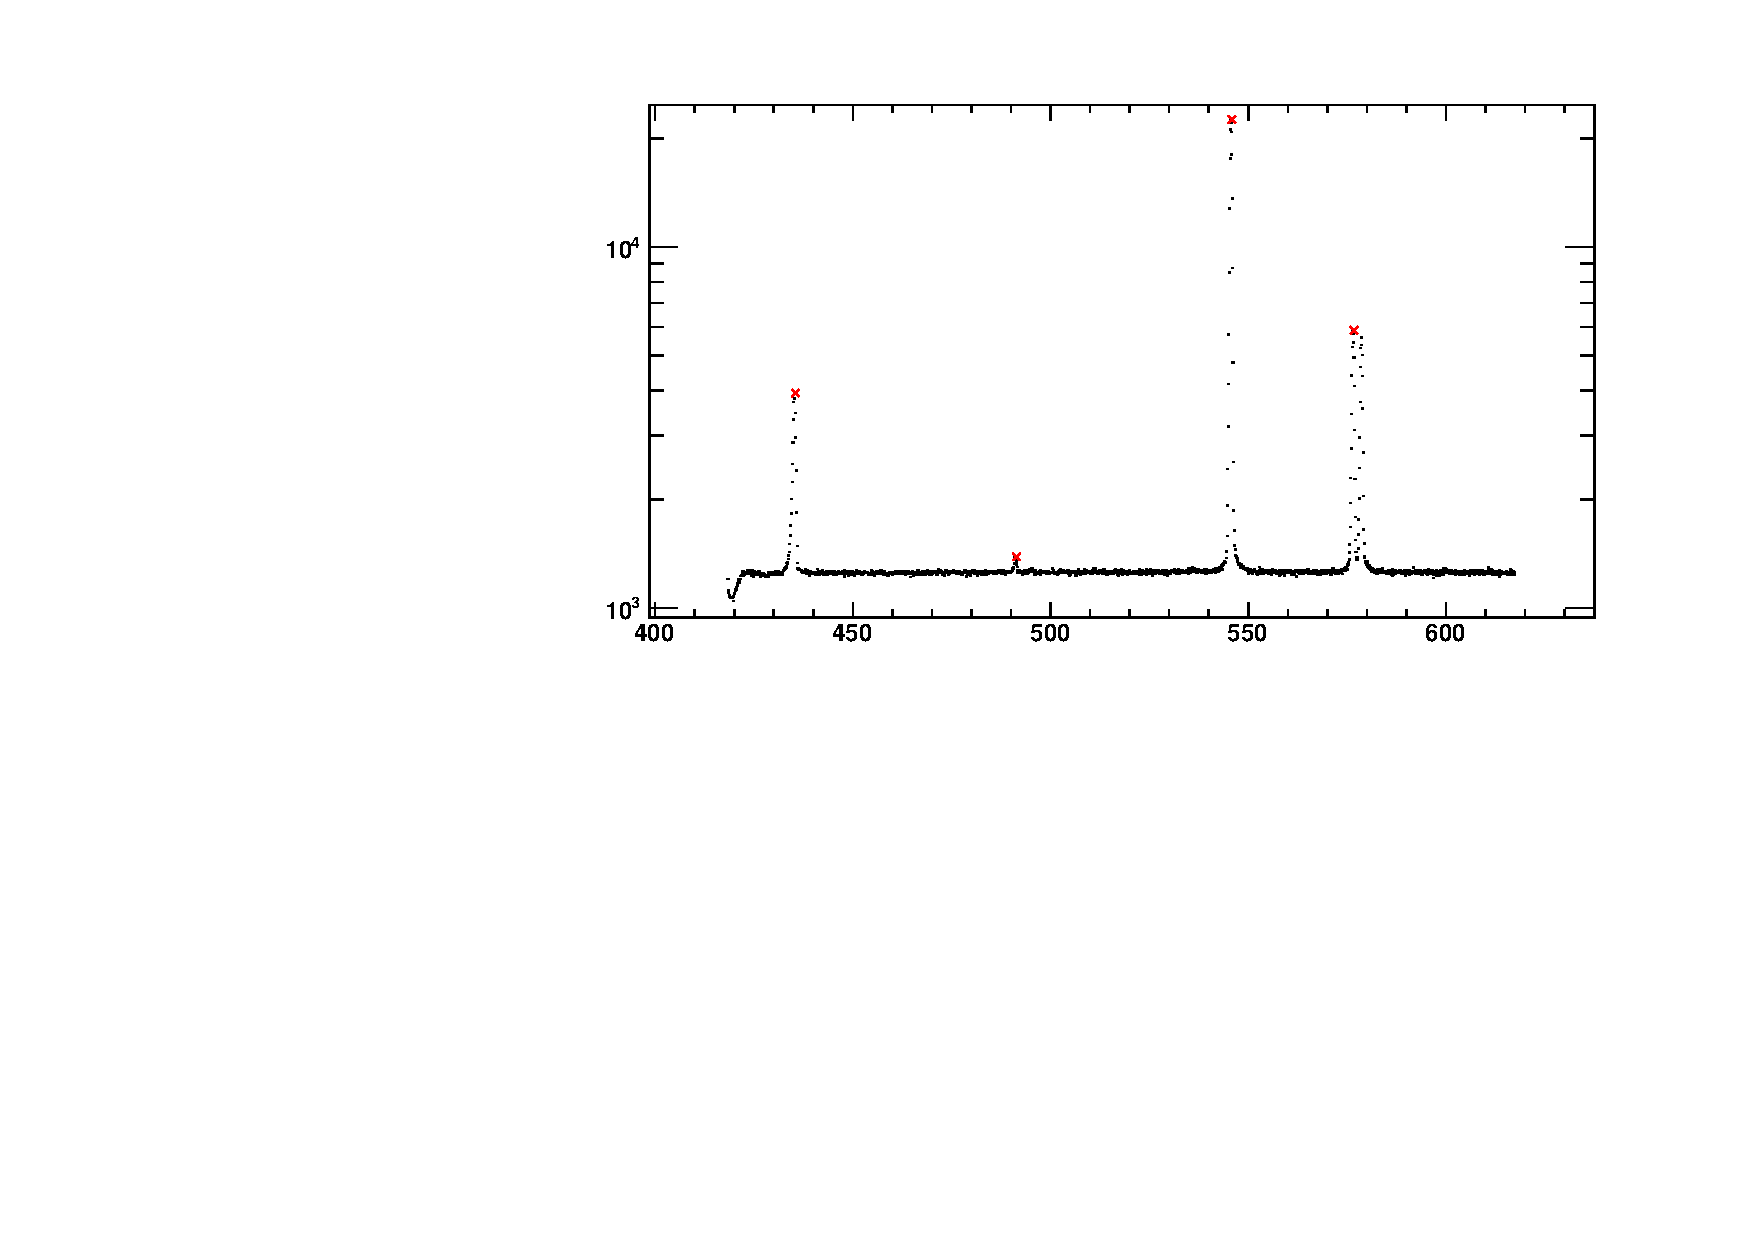
\includegraphics[width=\textwidth]{../img/HgPeaks.pdf}
  \caption[---]{Emission spectrum of Mercury with
  g-line at 435.83\,nm,
  e-line at 546.07\,nm and
  orange double lines at 576.96\,nm and 579.07\,nm.}
  \label{img:hg:spectrum}
\end{center}
\end{figure}

\begin{figure}[H]
\begin{center}
  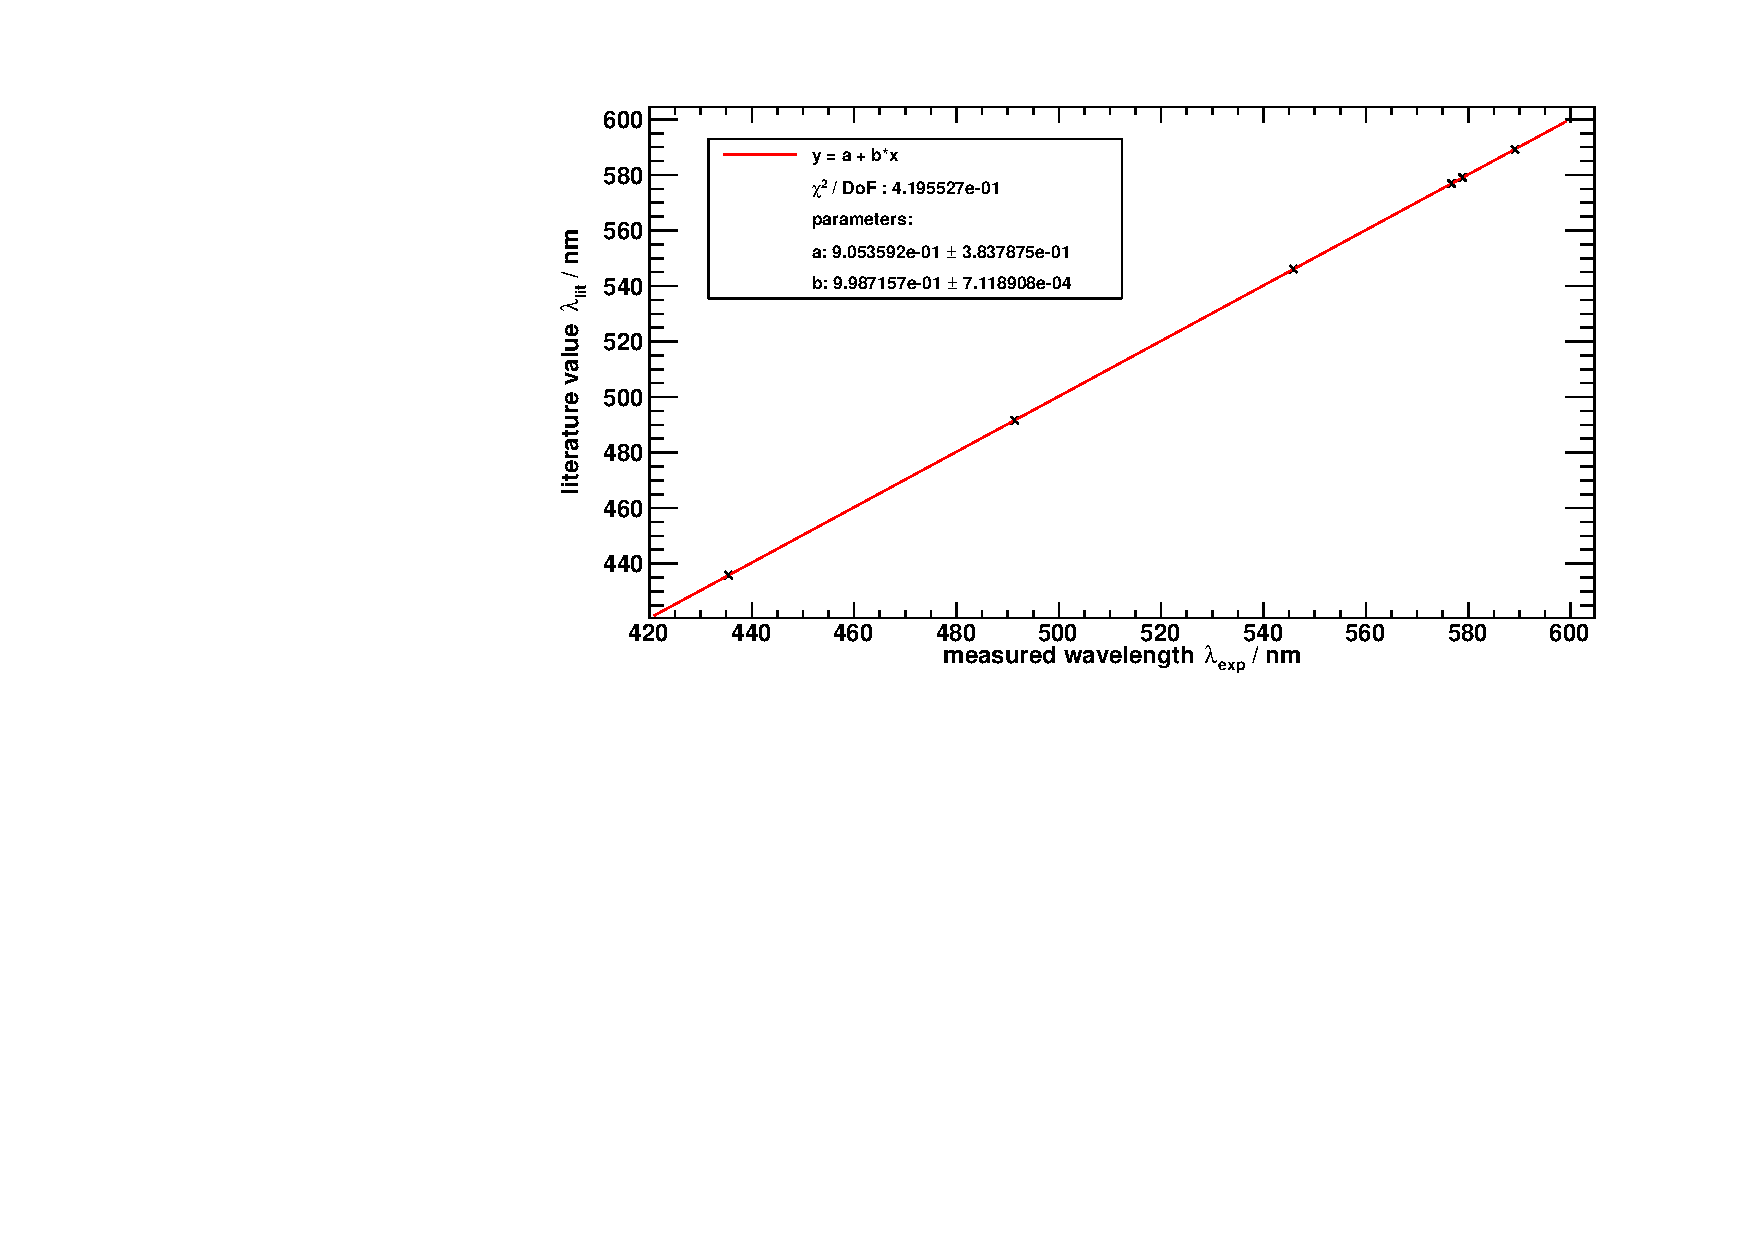
\includegraphics[width=\textwidth]{../img/energy_gauge.pdf}
  \caption[---]{Measured values for the lines of Sodium and Mercury versus literature values.
  The constant offset $a$ and the linear offset $b$ are used later to adjust the data of the iodine spectrum.}
  \label{img:calibrationsystem}
\end{center}
\end{figure}

\begin{figure}[H]
\begin{center}
  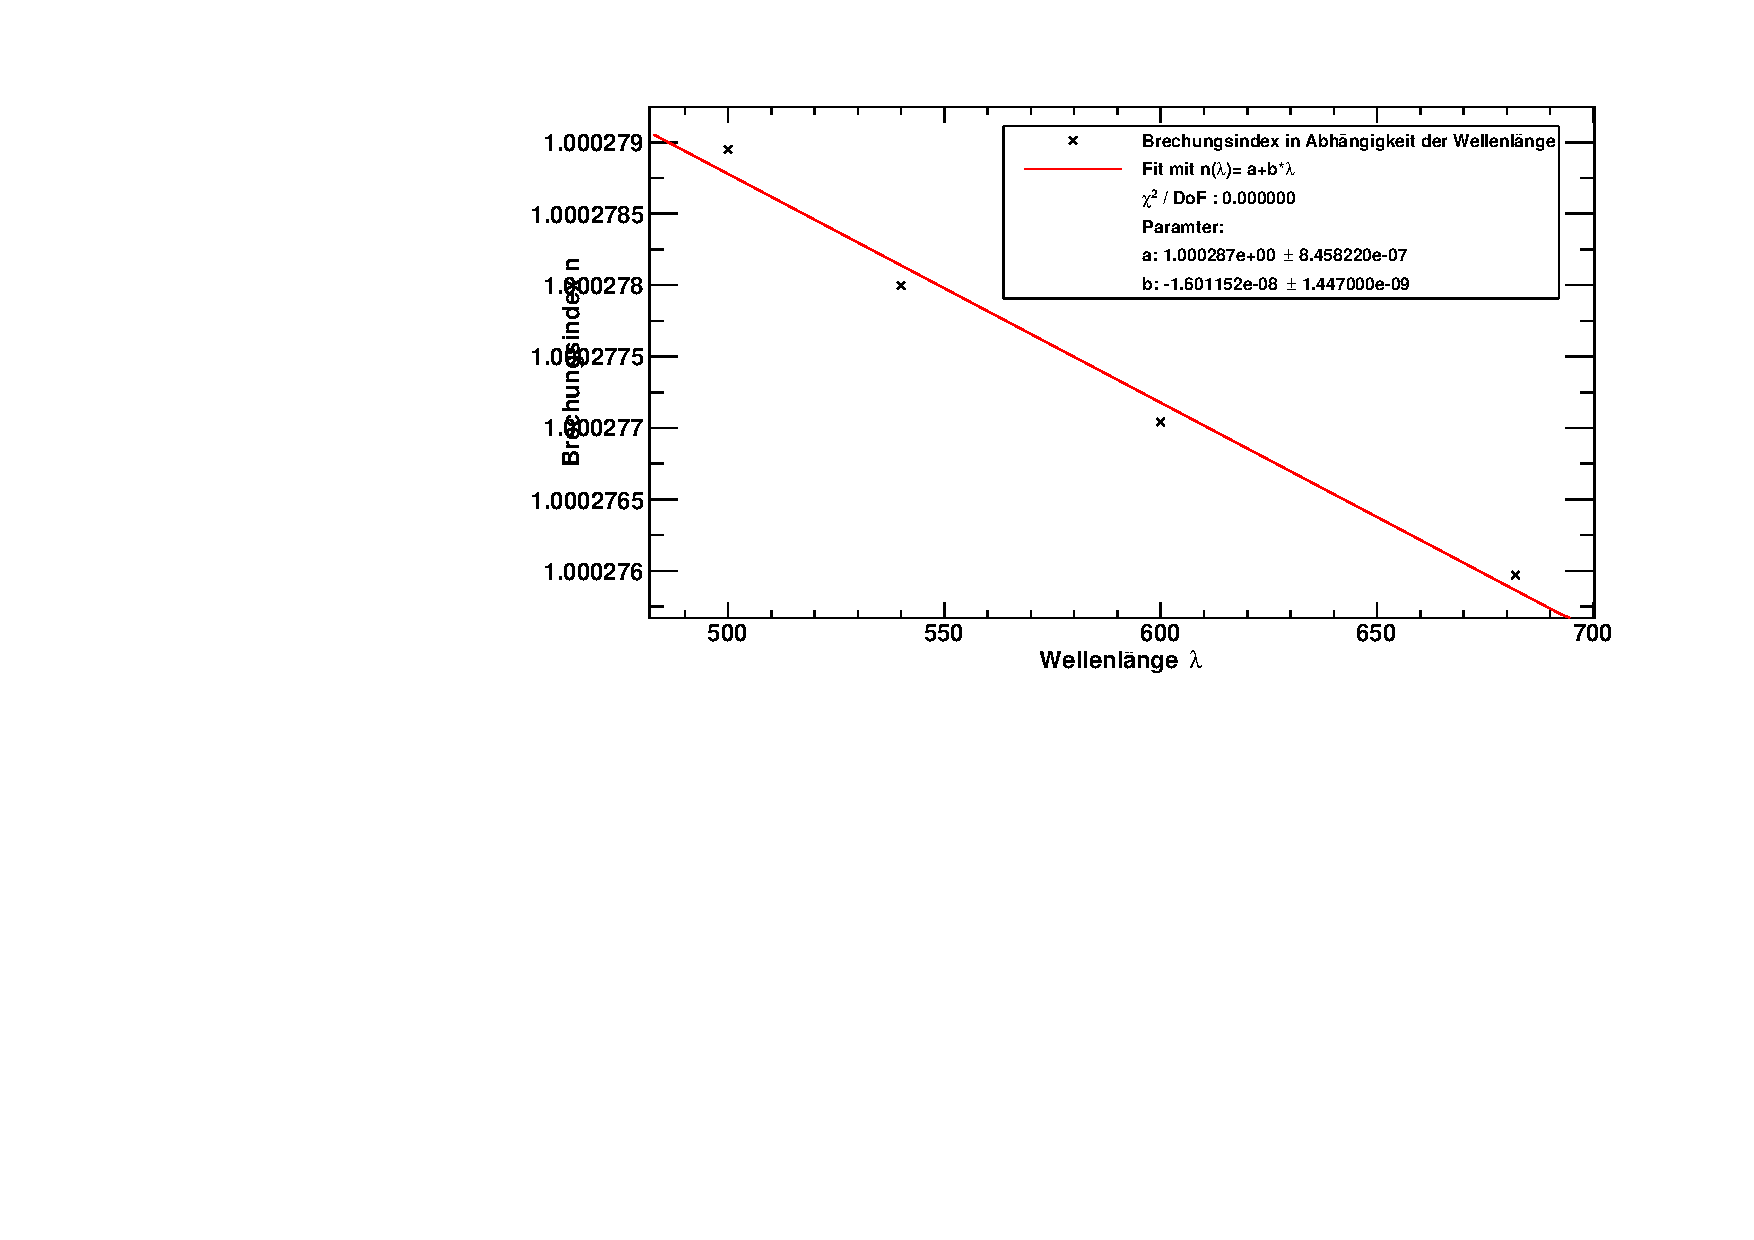
\includegraphics[width=\textwidth]{../img/fit_lambda.pdf}
  \caption[---]{Linear fit on the refraction index of air to obtain a function for adjusting
  the measured wavelengths to their vacuum value.}
  \label{img:refindex}
\end{center}
\end{figure}




\subsection{Spectrum of the halogen lamp}

\autoref{img:hal:spectrum} shows the spectrum of the halogen lamp.
The spectrum looks smooth an no absorption lines are visible.
An approximation with the model of a black body gives no good description of the data,
so probably the emissivity of the lamp changes for different wavelengths. 



\begin{figure}[H]
\begin{center}
  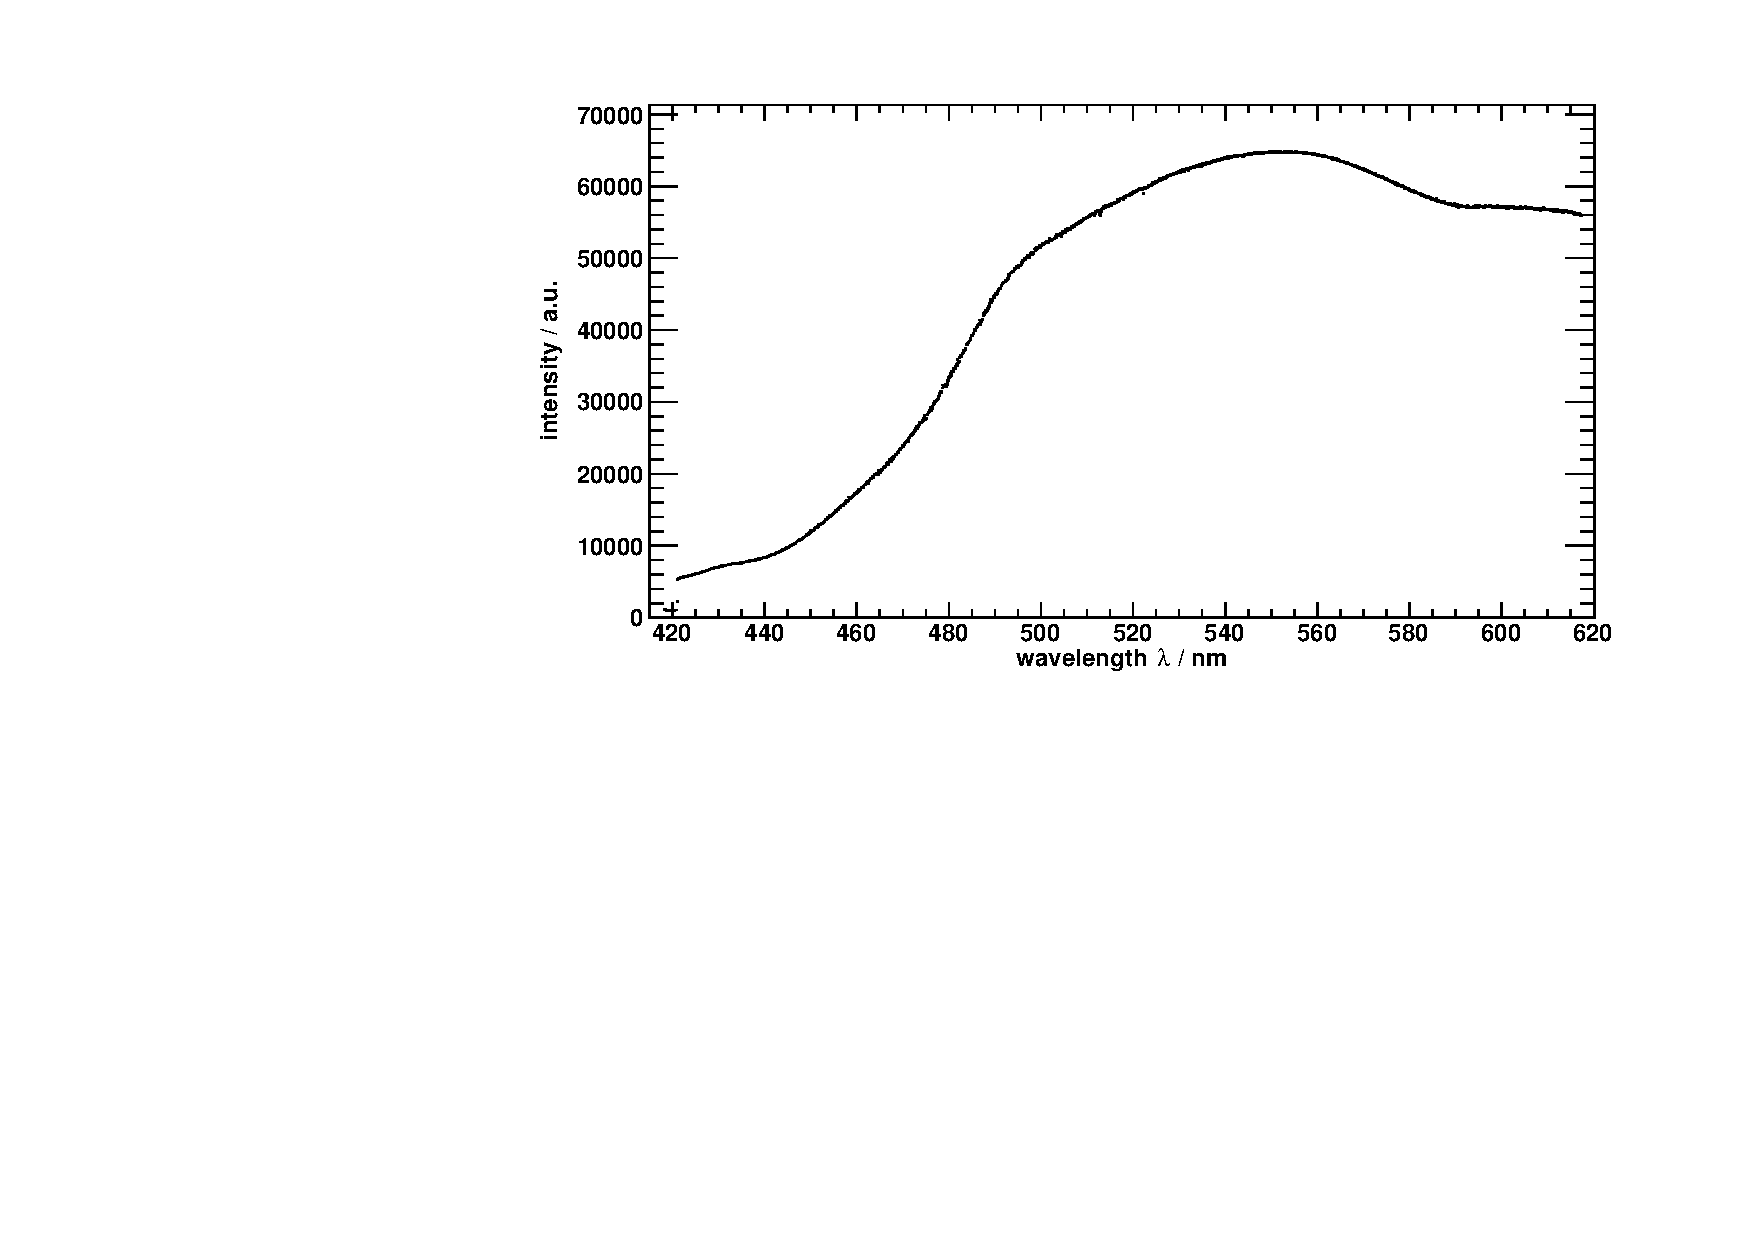
\includegraphics[width=\textwidth]{../img/halogen_lamp.pdf}
  \caption[---]{Spectrum of the halogen lamp.}
  \label{img:hal:spectrum}
\end{center}
\end{figure}




\subsection{Identification of the 3 progressions in the spectrum of iodine}

\begin{figure}[H]
\begin{center}
  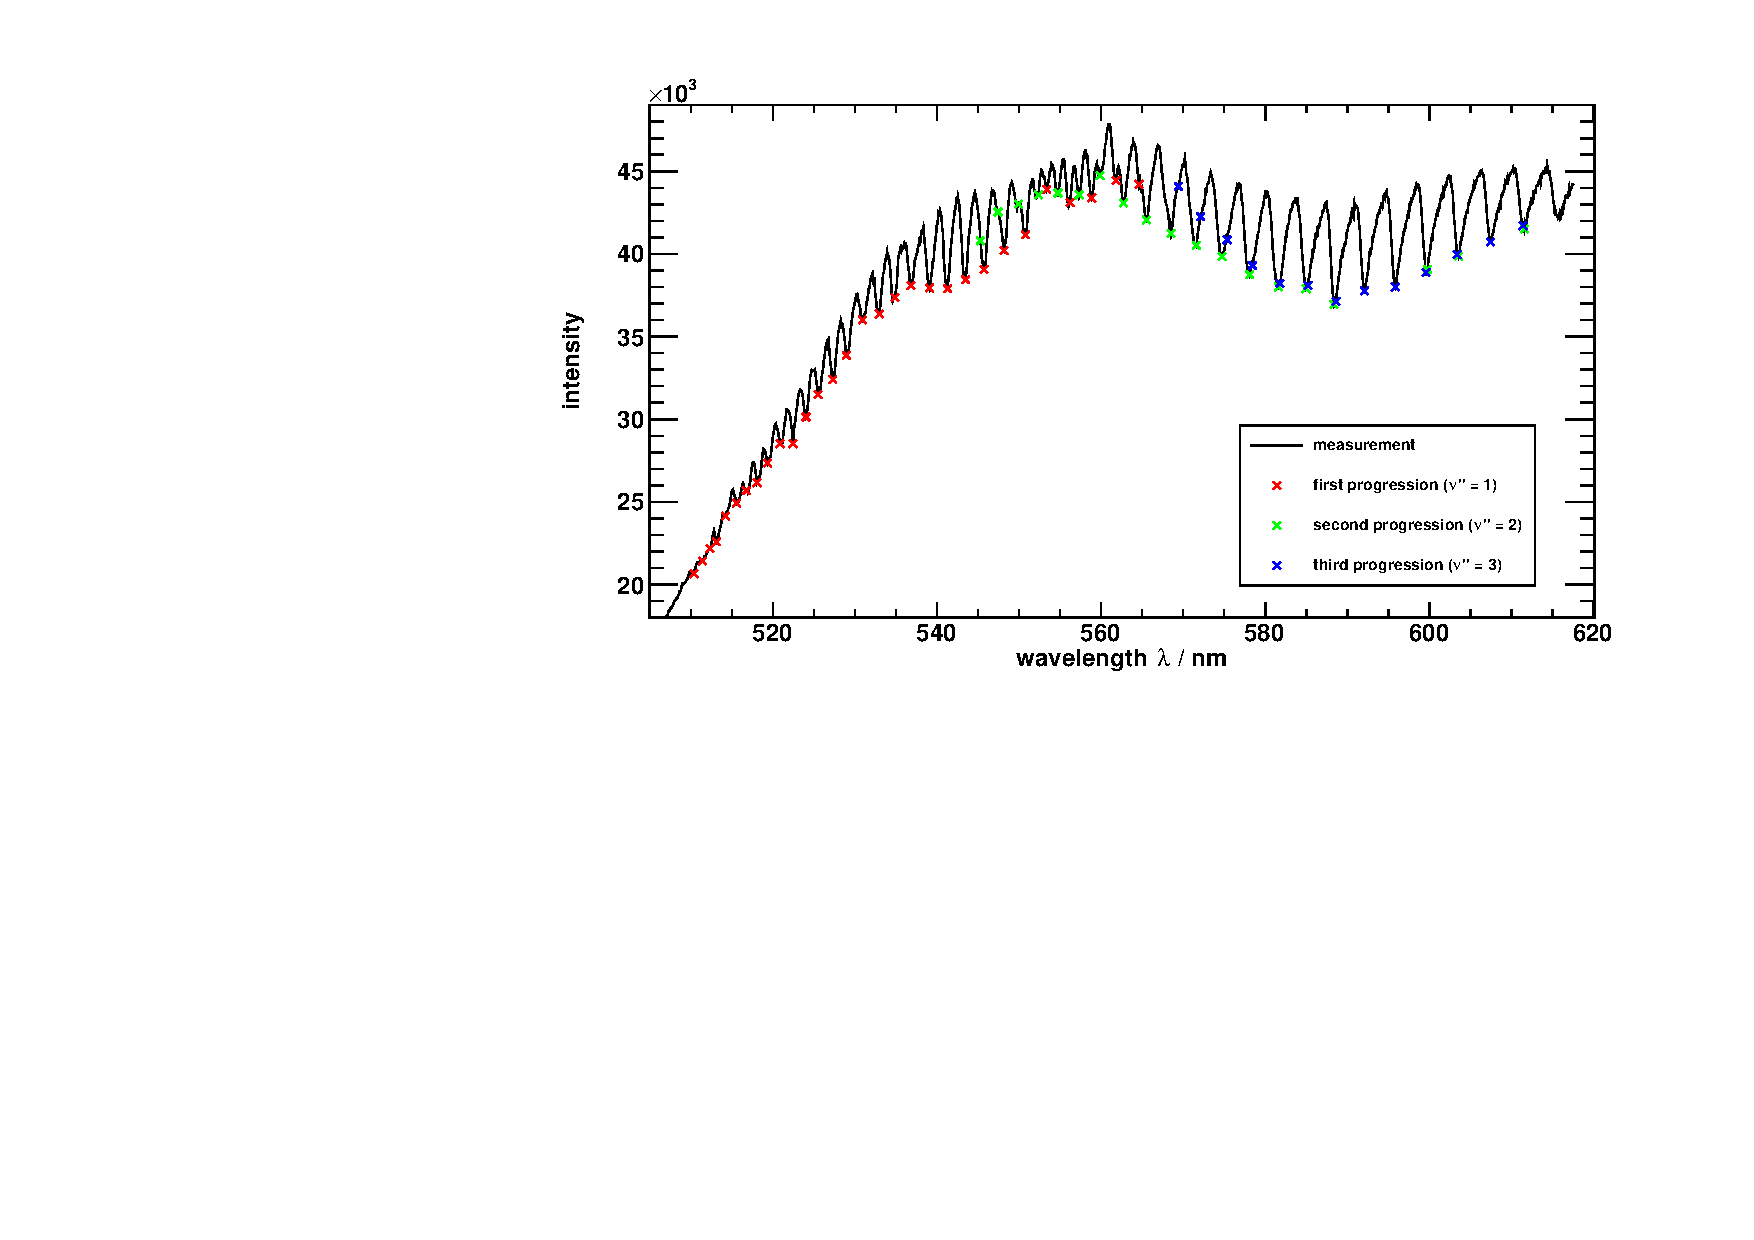
\includegraphics[width=\textwidth]{../img/I2_absorption.pdf}
  \caption[---]{Transmission spectrum of iodine and identification of absorption peaks due
  to electronic-vibronic transitions.}
  \label{img:spectrumiodine}
\end{center}
\end{figure}

\autoref{img:spectrumiodine} shows the measured transmission spectrum of a halogen lamp through iodine.
The first three progressions
(minima of transmission due to simultaneous electronic and vibronic excitation of iodine molecules)
could be identified and are marked in the
figure\footnote{The exact positions of the lines and
their corrected values (with calibration data of the setup and refraction index of air)
are shown in the Appendix, \autoref{tab:prog1}, \autoref{tab:prog2} and \autoref{tab:prog3}.}.
A closer look at the shape of those ''dips'' yields information about the ratio of the rotation constants
of the ground state and the excited electronic state:
The dips are slightly asymmetric and steeper on their left side. This so called
''red-shadowing'' appears, when the rotation constant of the excited state is \emph{smaller} than
the one of the ground state. As the constants are closely related to the equilibrium distance between the nuclei,
one can see that on excitation the nuclei move away from each other.

%TODO Nulllinie-Bandenkopf ???


\subsection{Evaluation of the oscillation constants $\omega_e'$ and $\omega_e' x_e'$ for the excited state
via Birge-Sponer plot}


\begin{figure}[H]
\begin{center}
  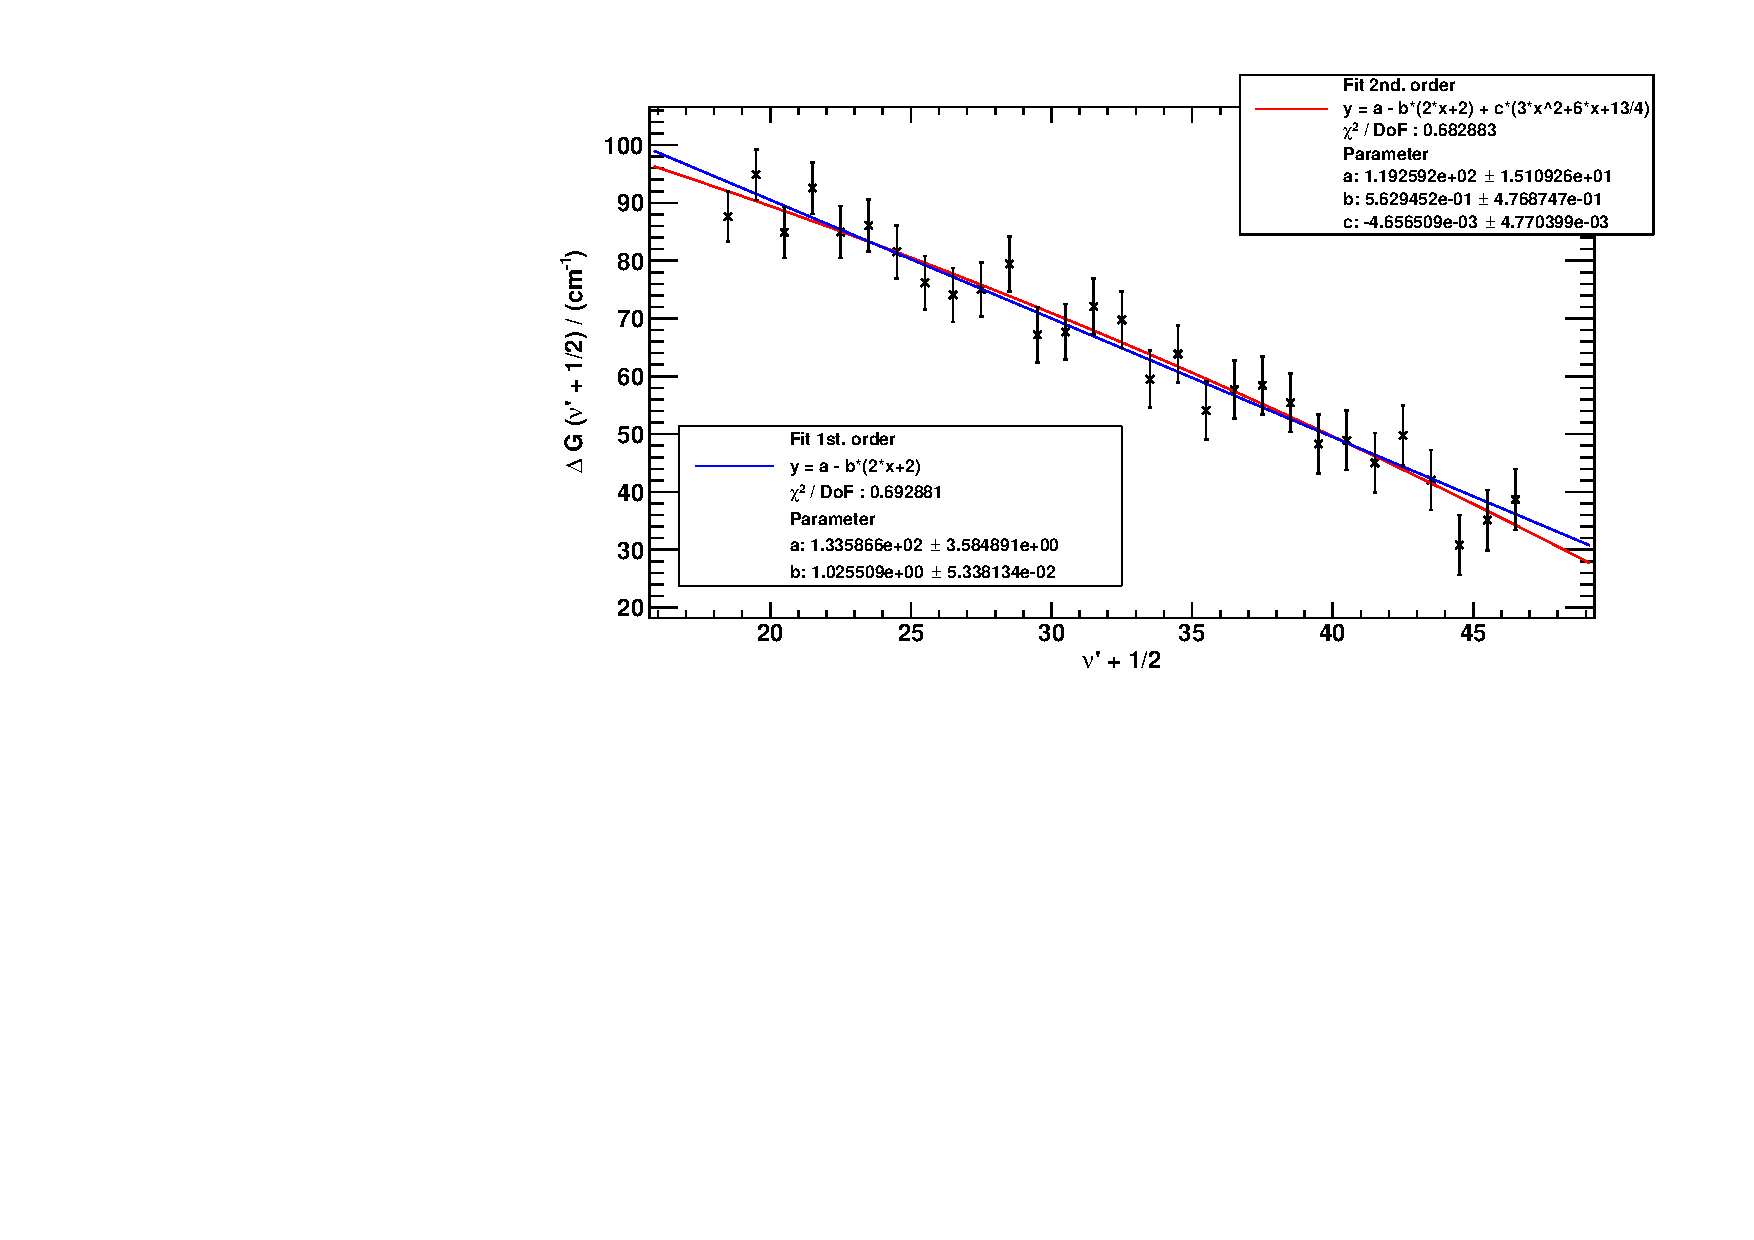
\includegraphics[width=\textwidth]{../img/prog1_birgesponer.pdf}
  \caption[---]{---}
  \label{img:prog1}
\end{center}
\end{figure}


\begin{figure}[H]
\begin{center}
  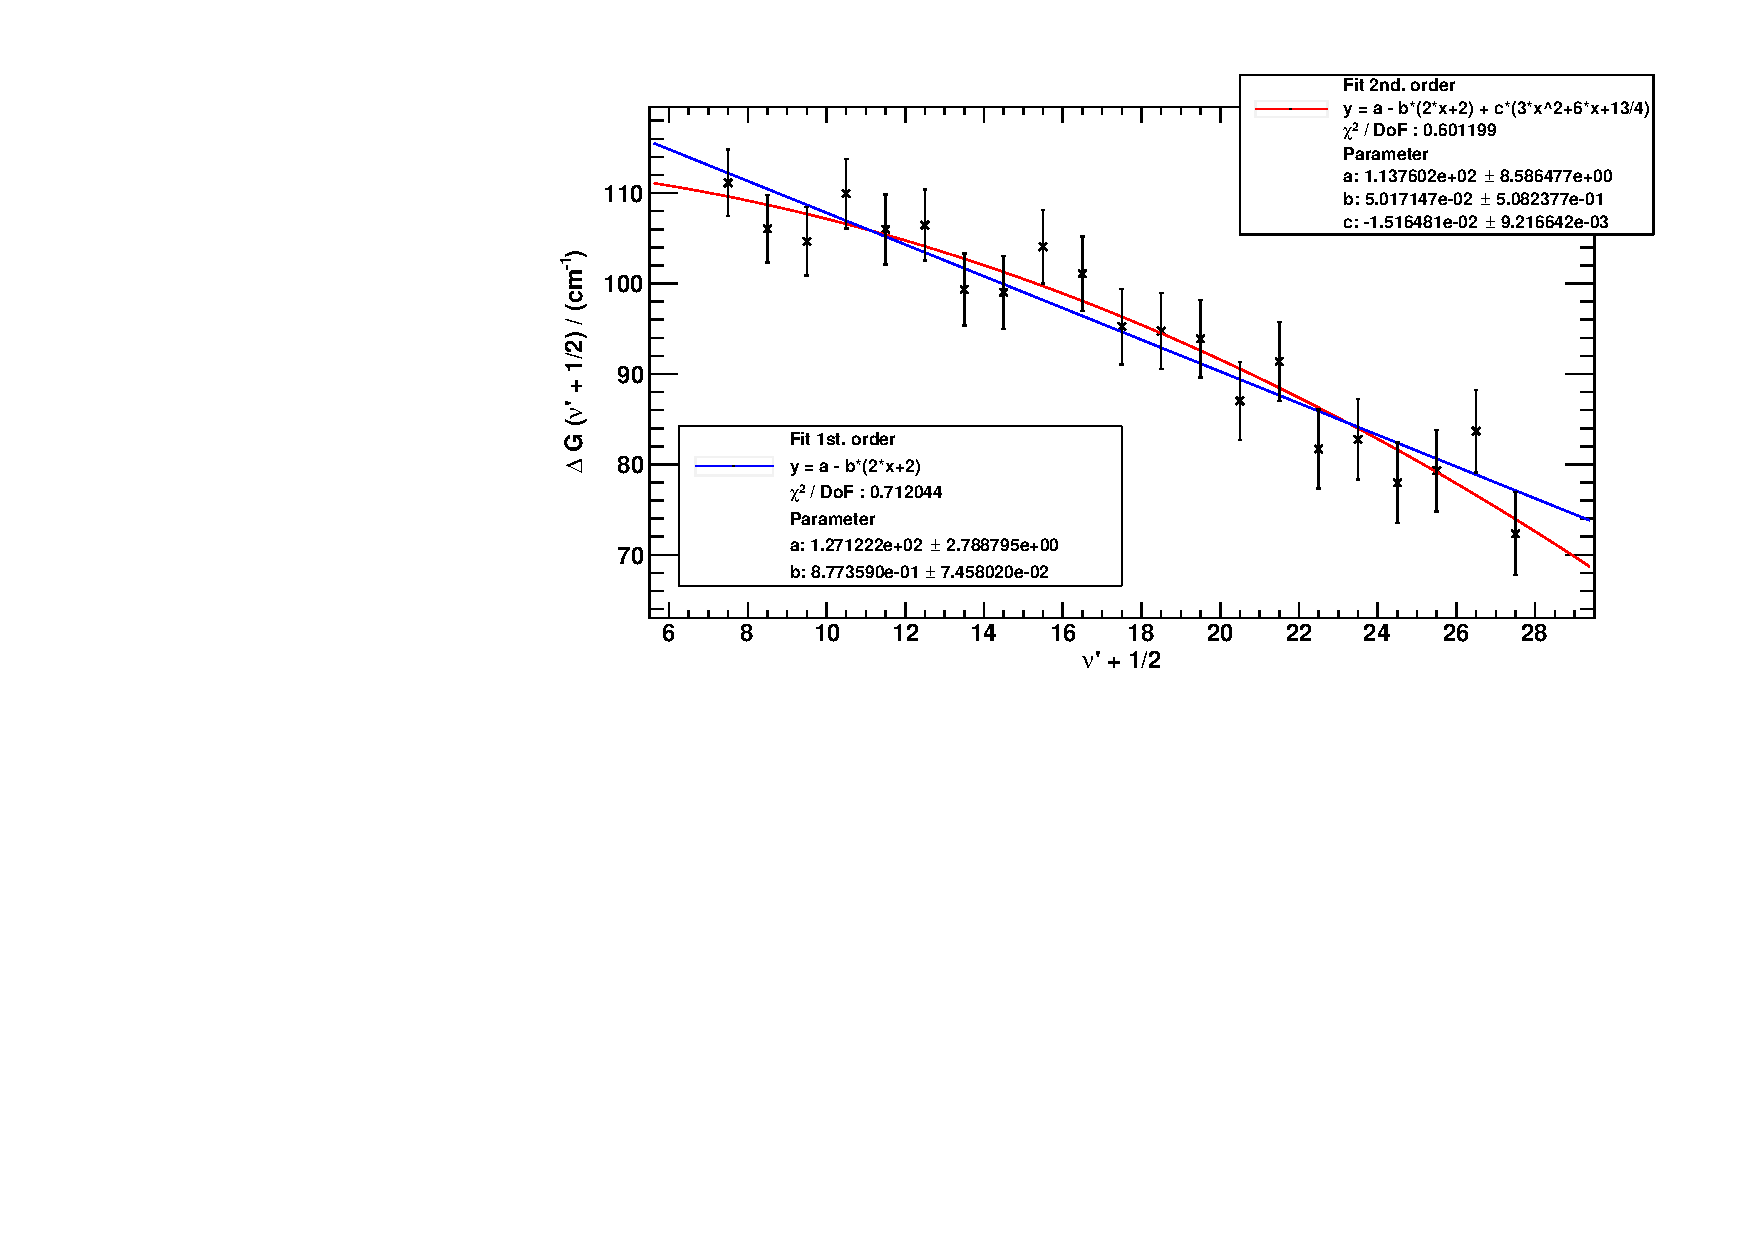
\includegraphics[width=\textwidth]{../img/prog2_birgesponer.pdf}
  \caption[---]{---}
  \label{img:prog2}
\end{center}
\end{figure}


\begin{figure}[H]
\begin{center}
  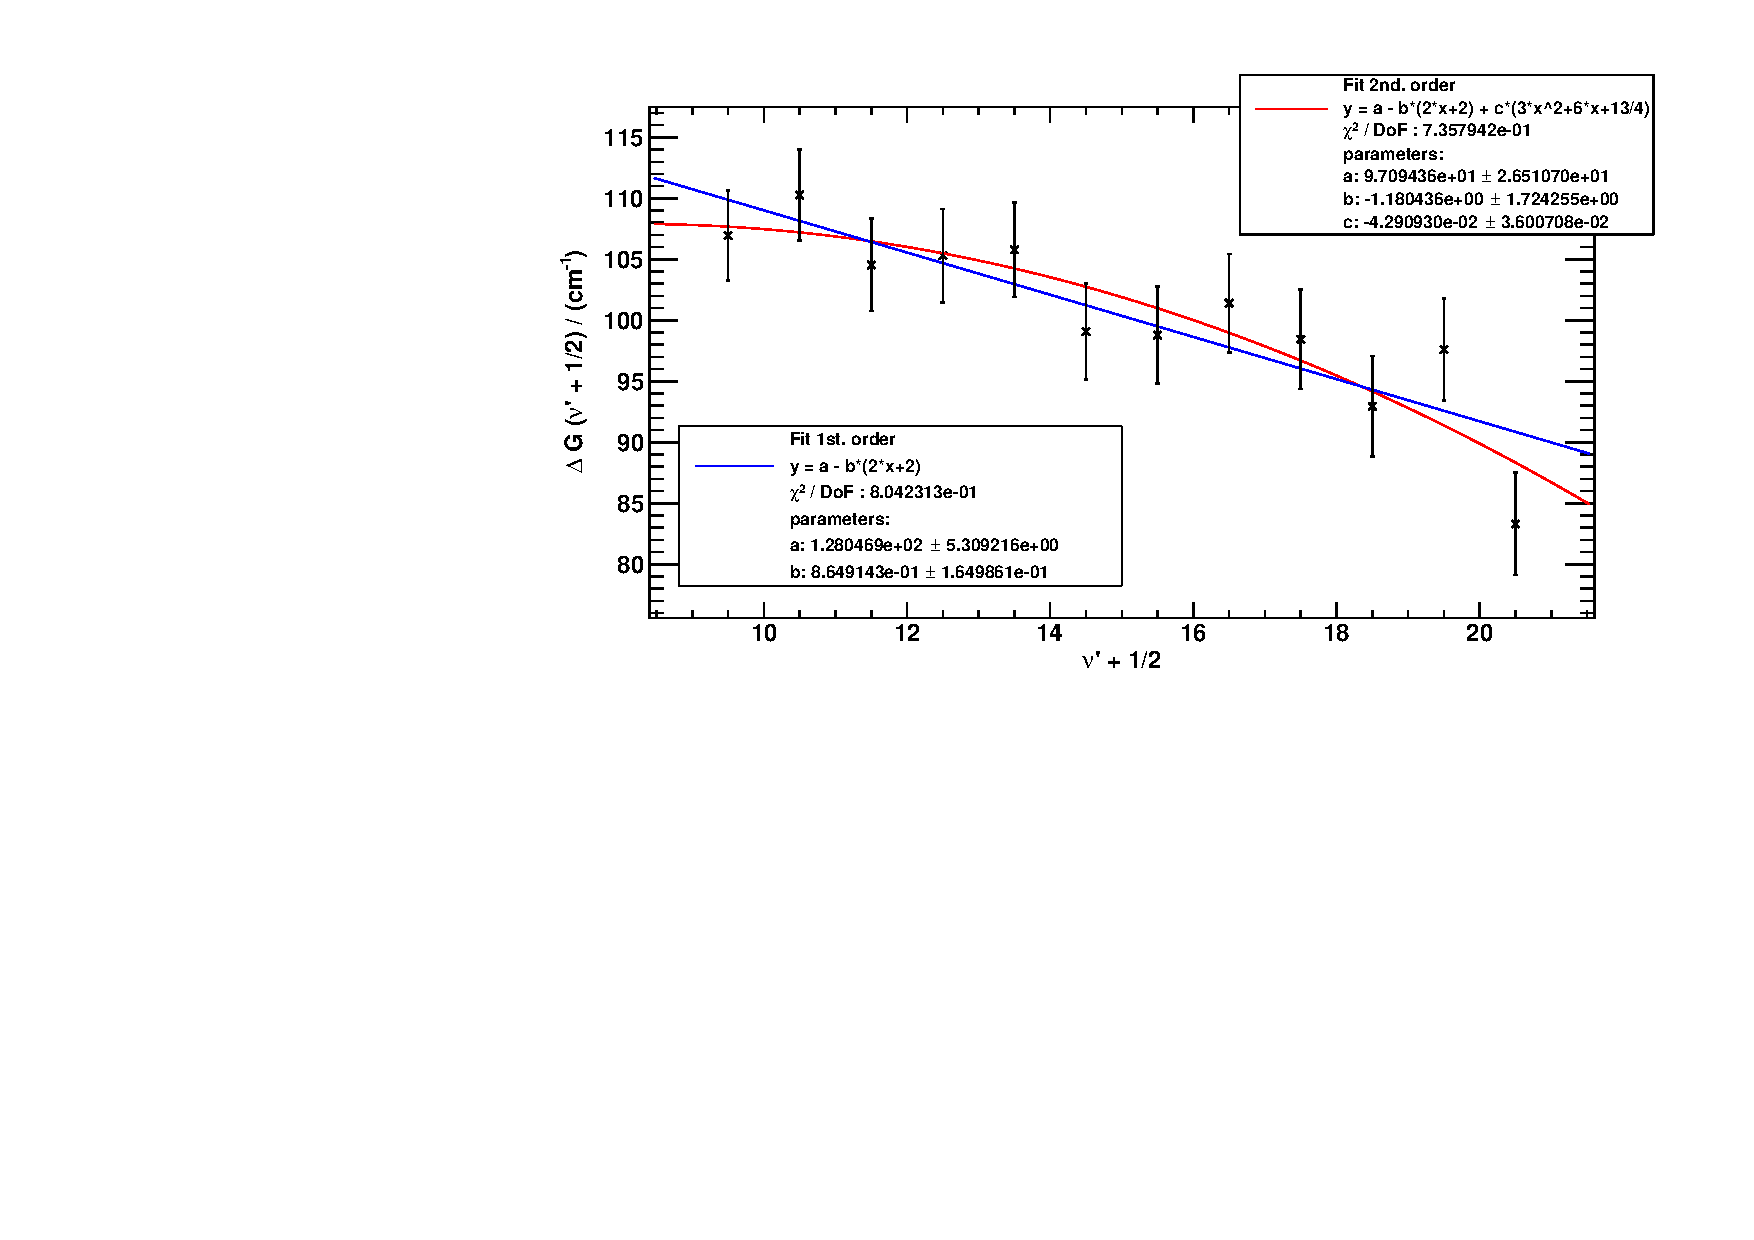
\includegraphics[width=\textwidth]{../img/prog3_birgesponer.pdf}
  \caption[---]{---}
  \label{img:prog3}
\end{center}
\end{figure}


\subsection{Evaluation of the oscillation constants $\omega_e''$ and $\omega_e'' x_e''$ for the ground state}



\subsection{Evaluation of the oscillation constants $\omega_e''$ and $\omega_e'' x_e''$ for the ground state}

\subsection{Determination of the dissociation energies}

\subsubsection{Via Morse-Approximation for ground state ($D_e''$) and excited state ($D_e'$)}

\subsubsection{Graphically from the Birge-Sponer plot for the excited state ($D_0'$)}

\subsubsection{Analytically for the ground state ($D_0''$)}

Graphik mit Energieniveaus

\subsection{Determination of the energy for electronic excitation $\sigma_{00}$}

\subsection{Morse potential for the excited state}


\begin{figure}[H]
\begin{center}
  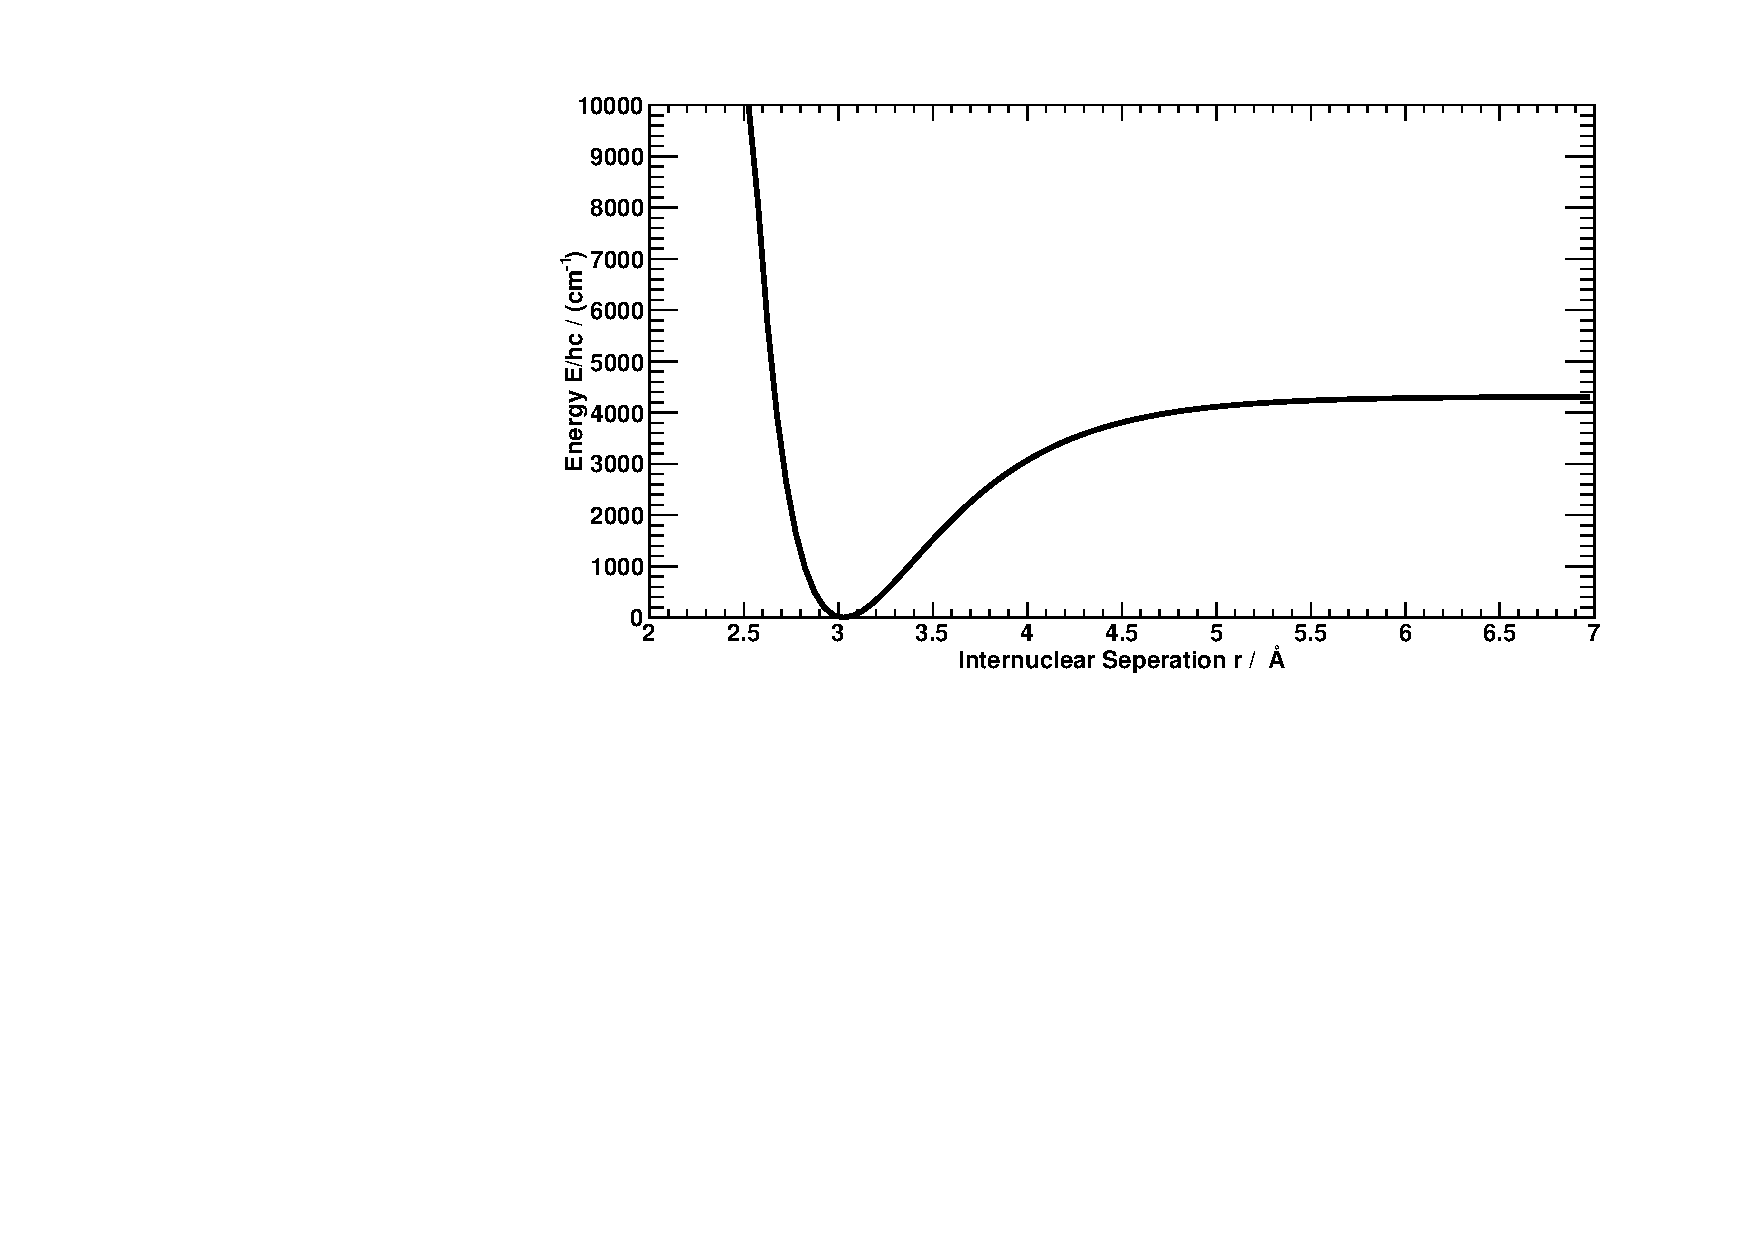
\includegraphics[width=\textwidth]{../img/morse.pdf}
  \caption[---]{---}
  \label{img:morse}
\end{center}
\end{figure}

